\section{Remote Vision Virtual Subsystem}%
\label{sec:remote-visi-subsyst-design}
The \glsfirst{rvvs} is mainly responsible for providing visual feedback to the
user of the vehicle's surroundings to assist its navigation. Additionally, it should offload the
\gls{nvs} from other intensive, but no so critical, tasks --- like
telemetry data --- as well as provide redundant paths for communications,
especially in the most critical conditions, like off-grid navigation with the
inclusion of the \gls{gprs} module. Thus, as aforementioned and illustrated in
Fig.~\ref{fig:initial-design-2}, it interfaces three different subsystems:
\gls{nvs} via RS232 communication; smartphone via Wi-Fi or \gls{gprs}; and the
web camera.

The \acrshort{rvvs} design was divided into three phases, corresponding to the
functional, object and dynamic models.
%
\subsection{Functional model}%
\label{sec:functional-model-rvvs}
The functional model describes the functionalities of the system from the
actors' perspective, illustrated in Fig.~\ref{fig:rvvs-use-cases-diag} by an use
case diagram. Two actors were identified: \gls{nvs} and Smartphone. The
Smartphone acts a proxy for user interaction, thus for clarity purposes, the
actor was named \emph{User}. Three main set of features were identified, namely:
\begin{enumerate}
\item \textbf{Communication}: deals with the communications interfaces between the
  various subsystems, further decomposed into the required functionalities for
  each interface (\emph{Comm Functions}). The \emph{User} may communicate with
  the \gls{rvvs} subsystem via GPRS or Wi-Fi, thus requiring the latter to
  provide network discovery capabilities, alongside with the conventional
  connect, send, receive and  disconnect functionalities. Additionally, it may
  also required periodic \textit{KEEP ALIVE} pings to check if the connection is
  still on. The \acrshort{nvs} communicates via RS232, which does not require
  network discovery. Lastly, the user may require sensor information, which
  could potentially be connected to the \gls{rvvs} subsystem (e.g., in a
  \gls{i2c} network) for offloading the \gls{nvs} subsystem.
\item \textbf{Image Acquisition}: responsible for providing visual feedback
  to the user. It can be configured, started, stopped and captured.
\item \textbf{Processing}: responsible for processing: user commands for image
  acquisition or forwarding them to the \gls{nvs} subsystem as a redundant path;
  telemetry data, such as, overall distance traversed, maximum speed so far,
  and operation time.
\end{enumerate}
% Use case diagrams
\begin{figure}[!hbt]
\centering
    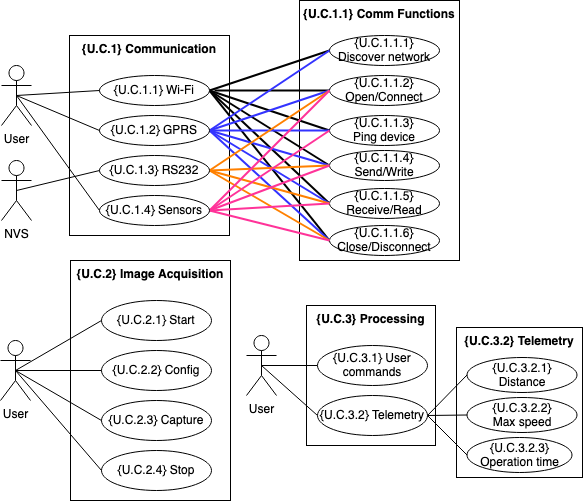
\includegraphics[width=0.7\textwidth]{./img/rvvs-use-cases-diag.png}
  \caption{Use case for \acrshort{rvvs} subsystem}%
\label{fig:rvvs-use-cases-diag}
\end{figure}
%%% Local Variables:
%%% mode: latex
%%% TeX-master: "../../../dissertation"
%%% End:
